\documentclass[tikz, border=10pt]{standalone}
\usetikzlibrary{arrows,positioning}

\begin{document}
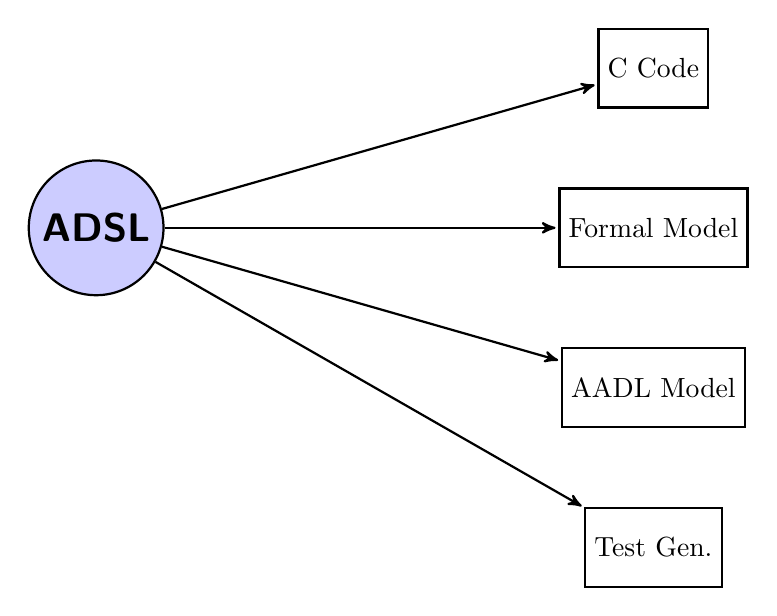
\begin{tikzpicture}[->,>=stealth',shorten >=1pt,auto,node distance=3cm,
  thick,main node/.style={circle,fill=blue!20,draw,
  font=\sffamily\Large\bfseries,minimum size=15mm},
  tar node/.style={rectangle,draw,minimum size=10mm}]

  \node[main node] (A)                   {ADSL};
  \node[tar node]  (M)  [right=5cm of A] {Formal Model};
  \node[tar node]  (C)  [above=1cm of M]     {C Code};
  \node[tar node]  (AA) [below=1cm of M]     {AADL Model};
  \node[tar node]  (TG) [below=1cm of AA]    {Test Gen.};

  \path[every node/.style={font=\sffamily\small,
        fill=white,inner sep=1pt}]
    (A) edge (C)
    (A) edge (M)
    (A) edge (AA)
    (A) edge (TG);

\end{tikzpicture}
\end{document}
